%%% LaTeX Template: Two column article
%%%
%%% Source: http://www.howtotex.com/
%%% Feel free to distribute this template, but please keep to referal to http://www.howtotex.com/ here.
%%% Date: February 2011

%%% Preamble
\documentclass[	DIV=calc,%
							paper=a4,%
							fontsize=12pt,%
							onecolumn]{scrartcl}	 					% KOMA-article class

\usepackage{lipsum}													% Package to create dummy text
\usepackage[brazil]{babel}										% English language/hyphenation
\usepackage[protrusion=true,expansion=true]{microtype}				% Better typography
\usepackage{amsmath,amsfonts,amsthm}					% Math packages
\usepackage[pdftex]{graphicx}									% Enable pdflatex
\usepackage[svgnames]{xcolor}									% Enabling colors by their 'svgnames'
\usepackage[hang, small,labelfont=bf,up,textfont=it,up]{caption}	% Custom captions under/above floats
\usepackage{epstopdf}												% Converts .eps to .pdf
\usepackage{subfig}													% Subfigures
\usepackage{booktabs}												% Nicer tables
\usepackage{fix-cm}													% Custom fontsizes
\usepackage[utf8]{inputenc}
\usepackage[top=2.5cm, bottom=2.5cm, left=2.5cm, right=2.5cm]{geometry}
\usepackage[ddmmyyyy]{datetime}
\addto\captionsenglish{%
	\renewcommand\tablename{Tabela}
	\renewcommand\figurename{Figura}
} 
 

 
%%% Custom sectioning (sectsty package)
\usepackage{sectsty}													% Custom sectioning (see below)
\allsectionsfont{%															% Change font of al section commands
	\usefont{OT1}{phv}{b}{n}%										% bch-b-n: CharterBT-Bold font
	}

\sectionfont{%																% Change font of \section command
	\usefont{OT1}{phv}{b}{n}%										% bch-b-n: CharterBT-Bold font
	}



%%% Headers and footers
\usepackage{fancyhdr}												% Needed to define custom headers/footers
	\pagestyle{fancy}														% Enabling the custom headers/footers
\usepackage{lastpage}	

% Header (empty)
\lhead{}
\chead{}
\rhead{}
% Footer (you may change this to your own needs)

%% ====================================
%% ====================================
%% mude o rodape  do projeto
%% ====================================
%% ====================================

\lfoot{\footnotesize \texttt{Cabeamento Estruturado} \textbullet ~Projeto - D.H.U Contabilidade e Assessoria LTDA}


\cfoot{}
\rfoot{\footnotesize página \thepage\ de \pageref{LastPage}}	% "Page 1 of 2"
\renewcommand{\headrulewidth}{0.0pt}
\renewcommand{\footrulewidth}{0.4pt}



%%% Creating an initial of the very first character of the content
\usepackage{lettrine}
\newcommand{\initial}[1]{%
     \lettrine[lines=3,lhang=0.3,nindent=0em]{
     				\color{DarkGoldenrod}
     				{\textsf{#1}}}{}}



%%% Title, author and date metadata
\usepackage{titling}															% For custom titles

\newcommand{\HorRule}{\color{DarkGoldenrod}%			% Creating a horizontal rule
									  	\rule{\linewidth}{1pt}%
										}

\pretitle{\vspace{-30pt} \begin{flushleft} \HorRule 
				\fontsize{50}{50} \usefont{OT1}{phv}{b}{n} \color{DarkRed} \selectfont 
				}

%% ====================================
%% ====================================
%% mude o titulo  do projeto
%% ====================================
%% ====================================

\title{Projeto de cabeamento estruturado da empresa D.H.U Contabilidade e Assessoria LTDA}					% Title of your article goes here

%% ====================================



\posttitle{\par\end{flushleft}\vskip 0.5em}

\preauthor{\begin{flushleft}
					\large \lineskip 0.5em \usefont{OT1}{phv}{b}{sl} \color{DarkRed}}
\author{Thiago Mitsuo Yamada}  	% Author name goes here


\postauthor{\footnotesize \usefont{OT1}{phv}{m}{sl} \color{Black} 
					\\Universidade Tecnológica Federal do Paraná - Câmpus Cornélio Procópio 								% Institution of author
					\par\end{flushleft}\HorRule}

\date{}																				% No date




%%% Begin document
\begin{document}
\maketitle
\thispagestyle{fancy} 	
\thispagestyle{empty}		% Enabling the custom headers/footers for the first page 
% The first character should be within \initial{}




%% ====================================
%% ====================================
%% mude o resumo  do projeto
%% ====================================
%% ====================================
\initial{O}\textbf{objetivo do projeto será a criação de uma estrutura completamente nova de cabeamento estruturado para a empresa D.H.U Contabilidade e Assessoria LTDA. Essa nova estrutura será composta por diversos computadores, além de servidores de aplicação e backup. Todos os computadores serão interligados a um domínio, controlados pelo Active Directory, oferecido pelo sistema operacional Windows Server. Os usuários serão vinculados a este controlador de domínio e possuirão acesso a um terminal service. O projeto abrange todo o levantamento de planta física, elaboração da planta logica, levantamento dos equipamentos de informática e o orçamento da implantação.  }

%% ====================================
\begin{figure}
	\centering
	\includegraphics{utfpr}
\end{figure}

\vspace{1cm}
\centerline{\textit{\textbf{\today}}}

\clearpage
    \renewcommand*\listfigurename{Lista de figuras}
\listoffigures

\renewcommand*\listtablename{Lista de tabelas}
\listoftables




\clearpage
\renewcommand{\contentsname}{Sumário}
\tableofcontents
\clearpage

%% ====================================
%% ====================================
%% Inicio do texto
%% ====================================
%% ====================================
\section{Introdução}
A empresa atualmente está transitando para uma nova instalação, com estrutura predial mais moderna, atendendo aos requisitos para o projeto de cabeamento estruturado. Na estrutura atual, a empresa não possui nenhum sistema de cabeamento estruturado, e com o aumento no quadro de funcionários, a rede tornou-se instável, com muitos problemas de conexão e baixa velocidade.

O quadro de funcionários conta com 8 funcionários, divididos nas áreas de pessoa física, pessoa jurídica, gerência e arquivo morto. Os equipamentos de TI são constituídos em 9 computadores, 1 roteador, 1 switch e 2 impressoras. 

O escopo do projeto constitui a instalação física de toda a parte do cabeamento e equipamentos de TI, além de sua configuração, documentação completa e testes funcionais, isentando da realização da certificação.

A expansão da empresa não será maior que 30 computadores.

\subsection{Benefícios}
Os benefícios com a introdução de uma estrutura de cabeamento estruturado resultará em maior estabilidade para a rede, além da facilidade na manutenção, segurança para os funcionários e clientes, a possibilidade da execução de aplicativos de forma remota e o aumento do desempenho das atividades da empresa. 

\subsection{Organizações Envolvidas}
Coloque o nome de todas as organizações envolvidas. Se for um projeto real, identifique quais as responsabilidades de cada uma das organizações. É comum que em um projeto de redes (cabeamento), temos várias organizações, sendo que cada uma delas com uma determinada responsabilidade.

Sugestão: crie uma tabela contento a relação delas.



\section{Estado atual}

Atualmente o estado da rede é composta por uma pequena estrutura, constituindo de 1 roteador, 9 computadores, 1 switch e os cabos cat5 para a conexão entre os equipamentos de TI.

As principais reclamações dos funcionários baseiam-se nos problemas quanto a estabilidade da conexão. Muitos dos aplicativos utilizados sofrem com a queda da conexão e dessa forma gerando transtornos para a finalização dos serviços. Além disso a manutenção é dificultada por não possuir uma estrutura organizada.

\section{Requisitos}

Os requisitos do projeto são:

1- Possibilidade de expansão da rede para compra de novos equipamentos;

2- Serviço de controle de usuários;

3- Bloqueio de acesso a sites com conteúdo inapropriado;

4- Serviço de segurança das informações trafegadas na rede;

5- Serviço de cópia de segurança dos dados utilizados;

6- Serviço de acesso remoto para uso de aplicativos.

\section{Usuários e Aplicativos}
A situação atual da empresa consiste no quadro de 8 funcionários, todos com computadores individuais e 2 impressoras. A estimativa da empresa que o número de funcionários possa crescer com a mudança de estrutura predial e de rede, por essa razão o projeto prevê a distribuição de 30 pontos de rede para suprir a demanda futura. 

\subsection{Usuários}
Os perfis de usuário são compostos por 8 funcionários, divididos em dois para o escritório de gerência, um para o arquivo morto, dois para o escritório de pessoa física e mais dois no de pessoa jurídica.

\subsection{Aplicativos}
Os aplicativos utilizados pelo escritório com uso intenso são:

- Pacote Office da Microsoft, principalmente o Excel e o pacote LibreOffice, utilizando o aplicativo Calc.

- Aplicativos destinados a declaração para Receita Federal, Receita Estadual, Municipais e para declarações trabalhistas.

Os demais aplicativos utilizados pelo escritório são de uso normal, com navegadores de internet.


\section{Estrutura predial existente}

O prédio de acordo com a planta física, é composto por um sobrado, possuindo na parte térrea três salas, uma destinada a sala de TI, contendo 12 metros quadrados, uma para o escritório de pessoa jurídica, possuindo 28 metros quadrados e um escritório de pessoa física, contendo 36 metros quadrados.

Na parte superior do prédio, encontra-se as salas de gerência e de arquivo morto, ambas possuindo 38 metros quadrados. O prédio todo conta com uma estrutura projetada para atender a demanda de um projeto de cabeamento estruturado, disponibilizando eletrodutos para o alojamento dos cabos de rede. Além disso, a estrutura predial disponibiliza os painéis para alocar os Patch Panel.

As possíveis distancias entre os pontos de rede não ultrapassarão 1 metro.
\section{Planta Lógica - Elementos estruturados}

\subsection{Estado atual}
Deve ter a planta atual, se for o caso

\subsection{Topologia}
Proposta futura, proposta após implantação.
Deve conter o diagrama da rede. Atente-se a redundância  e ligações truncadas.
Deve explicar todos termos e componentes utilizados nestas plantas. Por exemplo: entrance facility, work area, horizontal cabling, etc..

Todos os elementos das figuras devem ser explicados. 
Crie esboço da configuração dos racks e brackets. Explique cada um dos componentes. Você pode criar uma tabela contendo figuras dentro, ou criar uma tabela e incluí-la como imagem. Por exemplo, verifique a tabela \ref{tab1}.

\begin{table}[h!]
\centering
\caption{Exemplo de tabela explicativa}
\label{tab1}
\begin{tabular}{|l|l|l|}
\hline
\multicolumn{3}{|l|}{Figura na Tabela} \\ \hline
1        & Rack          & 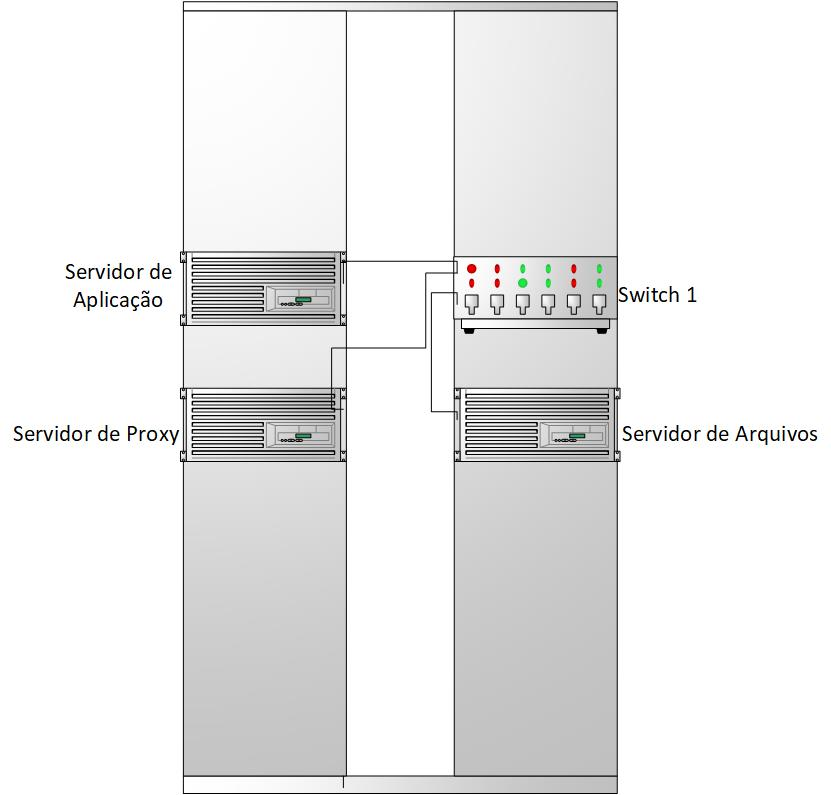
\includegraphics[scale=0.4]{rack1}        \\ \hline
2        & Rack 2        & 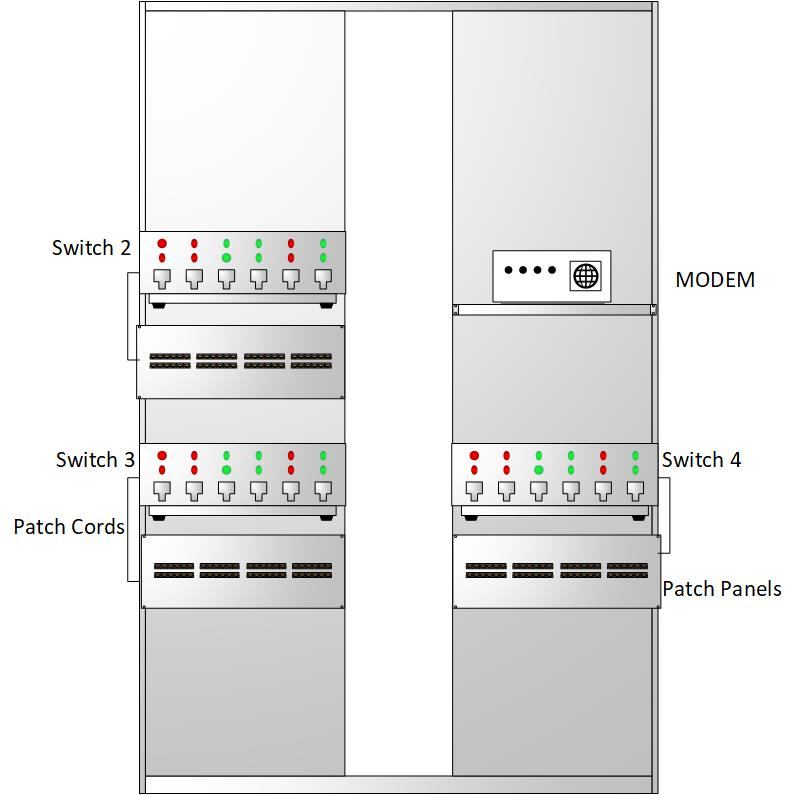
\includegraphics[scale=0.4]{rack2}        \\ \hline
\end{tabular}
\end{table}

\subsection{Encaminhamento}
Eletrodutos, calhas, e qualquer material em que os cabos serão alojados/alocados.

\subsection{Memorial descritivo}

Relacione todos os equipamentos passivos que serão utilizados, tipo, fabricante, quantidade.

\subsection{Identificação dos cabos}
Explique como os cabos serão identificados em seu projeto. Coloque uma relação dos cabos instalados e identificados.

\section{Implantação}
Estabeleça um cronograma de implantação:
Remoção de equipamentos existentes (destino para descarte), instalação dos condutores, instalação dos cabos, 
identificação dos cabos, montagem dos racks, certificação, etc... Crie atividades e estabeleça o tempo de execução. Se for um projeto real, indique também quais os responsáveis pela execução do projeto e de cada uma das etapas.

Defina marcas (e padrões) e fornecedores se for o caso. Atenção a contratados e subcontratados para a realização das atividades. Estabeleça a responsabilidade de execução da atividade e também da validação dela.

Utilize algum software para gerear o cronograma. Excel,etc. O fundamental é dividir em etapas, descrever e estimar o tempo de cada uma delas.

Segue uma relação de ferramentas:
http://asana.com/, 
https://trello.com/, 
http://www.ganttproject.biz/, 
http://www.orangescrum.org/. 

\section{Plano de certificação}
Quais seriam as etapas para a certificação? 
Quais os locais e horários para execução da certificação na rede? Toda rede será certificada?
Como os testes seriam executados?
Quais relatórios de certificação serão (ou deveriam ser) entregues? 

\section{Plano de manutenção}

Revisões periódicas na rede, emissão de certificados para novos pontos.

\subsection{Plano de expansão}
Existe um plano de expansão? Quantos novos pontos poderão ser acrecidos na rede, antes de migração de equipamentos na camada 2? Se houver expansão, quais equipamentos deverão ser direcionados para as estremidades da rede? 

\section{Risco}
Enumerar e explicar os riscos do projeto.

\section{Orçamento}
Crie uma relação de orçamentos baseado na seções anteriores.

\section{Recomendações}
Observações e recomendações para o cliente.

\section{Referências bibliográficas}
Utilize o mendley, o jabref ou diretamente o bibtex para gerenciar suas referências biliográficas. As referências são criadas automaticamente de acordo com o uso no texto.

Exemplo: Redes de computadores, segundo \cite{t2013} é considerada..... Já \cite{kurose2010} apresenta uma versão...

Analisando os pressupostos de \cite{ref3} e \cite{ref4} concluimos que....


\renewcommand\refname{} %%Referências bibliográficas}  
\bibliographystyle{ieeetr}
\bibliography{referencias}  

%% ***********************************************************************
%% === remover daqui =====================================================
%% ***********************************************************************
=================================================
\section{Elementos textuais - Alguns exemplos}

Esta seção apresenta exemplos de elementos textuais. \textbf{Remova-a da versão final do texto}.


\subsection{Colocar elementos em itens}

Texto antes da lista

\begin{itemize}
	\item First item in a list 
	\item Second item in a list 
	\item Third item in a list
\end{itemize}

\subsubsection{Uma subseção de terceiro nivel}

Exemplo de uma subseção

\subsection{Tabelas}

Utilize o site http://www.tablesgenerator.com/ para elaborar as tabelas de seu trabalho.
Para adicionar uma tabela utilize: a tag input, passando o arquivo da tabela como parametro

\input{tab2}

Dentro do arquivo você deve definir o label e pode utilizá-lo para referenciar. Exemplo:
Na tab \ref{tab2} temos a relação de ....


Você também pode modificar a tabela manualmente, incluindo, por exemplo h! dentro de sua definição. Veja no exemplo tab2.tex

\subsection{Figuras}

As figuras podem ser no formato PDF, JPG, PNG. Você pode referenciá-las da mesma maneira que tabelas. Exemplo: A figura \ref{fig1} apresenta.....

Não se preocupe o local em que a figura será renderizada em seu texto. Preocupe-se em criar referência para ela, ou seja, toda figura e tabela deve conter pelo menos uma referência no texto.

\begin{figure}
\centering
\includegraphics[width=\textwidth]{fig1}
\caption{Exemplo de figura com escala horizontal}
\label{fig1}
\end{figure}


\begin{figure}
	\centering
	\includegraphics[]{fig2}
	\caption{Exemplo de figura sem escala}
	\label{fig2}
\end{figure}

Você pode rotacionar figuras também. Para isso utilize o parâmetro angle=-90. Repare que a escala da figura foi modificada pelo parametro height. Você também pode utilizar scale

\begin{figure}
	\centering
	\includegraphics[height=\textwidth,angle=-90]{fig3}
	\caption{Exemplo de figura rotacionada}
	\label{fig3}
\end{figure}


%% ***********************************************************************
%% === ate aqui    =====  ================================================
%% ***********************************************************************

\end{document}